To carry out the 3D map of a Martian rock, the coordinates of the points which are projected by the LED on its surface need to be determined on the video stream of the camera. They are obtained by detecting the points thanks to their color, and by applying the centroid algorithm to get their center. First, the color detection method will be addressed, before focusing on the centroiding.

\subsection{Color Detection}

To increase the robustness of the algorithm, the color of the light beams was chosen to have the maximum contrast with the color of the rock. Mars having a reddish color, a bright green light seemed adapted. Moreover, as it is explained in the scene analysis part, the CCD sensor is more sensitive to the wavelength corresponding to the green (around 520 nm). Thus, the color detection algorithm aims to find bright green spots in the camera video stream in real time. It is implemented in C with OpenCV library. 

The image analysis is performed by extracting frames from the video stream. These images are processed very quickly, which allows a real time analysis. The details of the method employed are given below. For the explanation, the figures are obtained for the detection of a blue box, but the algorithm works similarly for green light beams.

To begin with, a low-pass filter is applied to the image to handle to smooth it and to reduce the noise. Once achieved, the image is converted from RGB to HSV (see Theory Section) in order to get a better control of the colors and intensities of the image pixels. The range of the HSV parameters can be determined to isolate the bright green pixels from the rest of the image. The equivalent hue is between 60\degree  and 180\degree, taking a large scope to be sure to isolate the good color component. As the luminous points will be bright, the range of the saturation and the luminosity should be chosen around the upper values. To adjust the values, several trackbars are added to the image, see figure \ref{fig:trackbars} and the modifications are made in real time. All the values under the threshold defined are irrelevant. Thus the pixels of the binary image which corresponds to the HSV thresholding are set to 1 (white) for the zone where the light beams are recognized and to 0 (black) for the background, the rest of the image. This image is then easier to deal with because it is only composed of two values, black and white. Erosions and dilations can be applied respectively to separate connected light beams and remove noise or to fill holes in the rays. The number or erosions and dilations are selected thanks to trackbars once again (figure \ref{fig:trackbars}) and they are computed with the OpenCV functions. 

\begin{figure}[H]
  \centering
  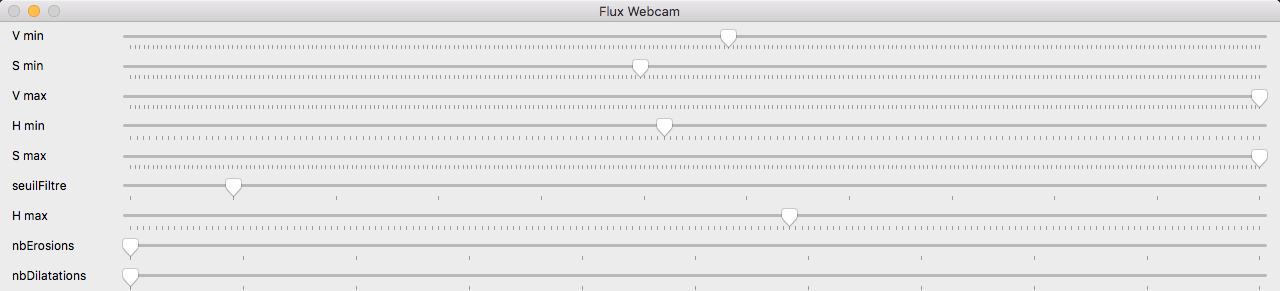
\includegraphics[scale=0.35]{fig/trackbars.png}
  \caption{Trackbars for the threshold of the filter, the HSV parameters and the number of erosion and dilation}
  \label{fig:trackbars}
\end{figure}

The calibration is carried out through the trackbars and the result is displayed on the video stream with the addition of contours to facilitate the tuning (figure \ref{fig:contours}). \textit{cvFindContours} is used to search the contour of the light beams. The detection is based on the same principle that it has been seen during the exercises in the lab. The algorithm looks for the first pixel belonging to the beam and then follows the contour pixel by pixel. Once the threshold of the low-pass filter, the HSV values and the number of erosion and dilation are established, the calibration is completed.

\begin{figure}[H]
  \centering
  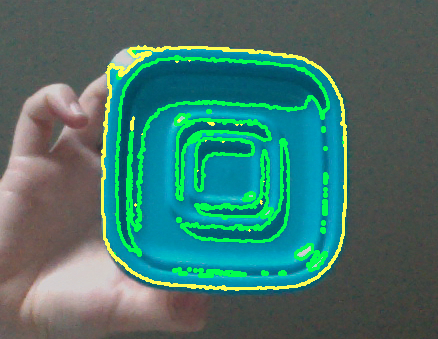
\includegraphics[scale=0.6]{fig/contours.png}
  \caption{Contours of the detected object}
  \label{fig:contours}
\end{figure}

In order to compute the centroid of the beams, it is needed to retrieve their intensity. To this end, the color detection should return an image with the light points in HSV color on a black background. To do so, the binary image is multiplied by the HSV image. The multiplication is explained by the pseudo code below. 

\begin{algorithmic}
\Function{multiplication}{binary image, color image}
	\For{each pixel in the binary image}
		\If {the pixel value is white}
    			\State $pixelHSVColor \gets$ the color of the pixel in the HSV image
    			\State the color of the pixel in the final image $\gets pixelHSVColor$
		\Else
        			\State the color of the pixel in the final image $\gets$ black color
		\EndIf
	\EndFor
\EndFunction
\end{algorithmic}

The final image obtained is shown figure \ref{fig:finalImage}.

\begin{figure}[h]
  \centering
  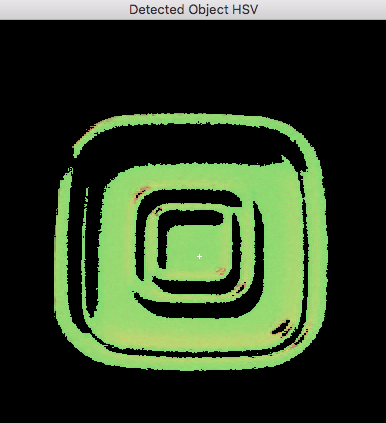
\includegraphics[scale=0.6]{fig/finalImage.png}
  \caption{Object detected in HSV color system on a black background}
  \label{fig:finalImage}
\end{figure}